\documentclass[../main/main.tex]{subfiles}

\newdate{date}{23}{04}{2020}

\begin{document}

\section{Lecture 14}
 \displaydate{date}. Compiled:  \today. Rachele+Alice.

\subsubsection{Slide 218}

\begin{figure}[h!]
\centering
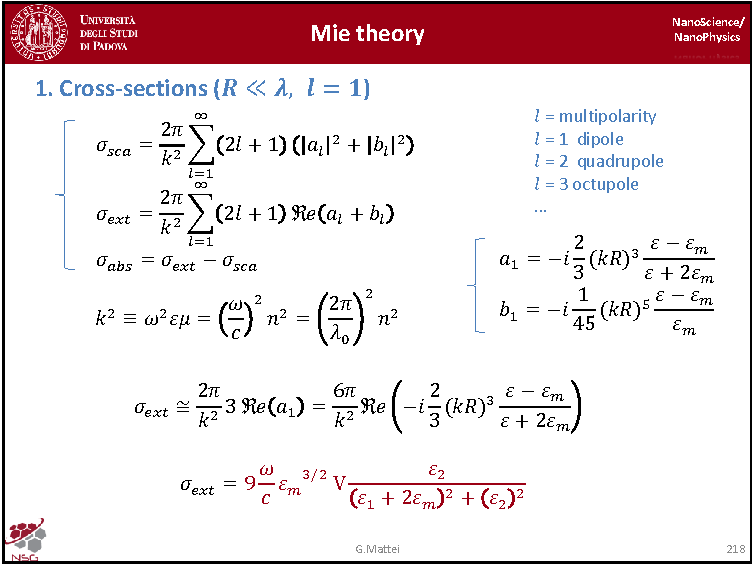
\includegraphics[page=1,width=0.9\textwidth]{../lessons/pdf_file/14_lesson.pdf}
\end{figure}

Previously, we have seen how to develop the full Mie theory in the full multipolar version, which is able to handle the quite complex problem of the interaction between a plane wave and a single isolated nanoparticle with arbitrary composition and embedded in a medium which is not absorbing.
With these assumptions, we were able to derive the solution of Helmholz equations for the electric and the magnetic field, for the internal field and scattered field at any level of accuracy as far as the multipolarity is concerned.

As we have seen, for the far field properties, like the scattering cross-section, we can use the tecnique of calculating the flux of the pointing vector, which is built out of the scattered electric and magnetic field, so we can build all the energy budget and the power budget that is delivered from the nanoparticles toward the far field, that is at large distance with respect to the wavelenght from the nanoparticle (that is things we can measure in real world).

We have seen that e scattering cross-section can be written with these equations and in particular when the multipolarity $l=1$ can be used (that is when the size parameter \( k R \) is much less than one or equivalently when R is much less than the wavelength) we can safely neglect $b_1$, and we can use just the multipolarity \( a_1 \), which is the dipolar component of those equations.
If we substitute in those equations, the relations for \( a_1 \) and \( b_1 \) from full Mie theory, we can realized that when the \( k R \) is much less than one, we can neglect \( b_1 \).
We remind that \( a_1 \) and \( b_1 \) are the coefficients which are used for the scattered field that is the most important quantity that we need.
If we neglect \( b_1 \), the extinction cross-section can be rewritten as (1), which is a restatement of the previous expression. If we put the explicit expression of $a_1$ we obtain the full extinction cross-section in the dipolar approximation (the formula in red, which is the most famous of the Mie theory).


In this case we have the resonant behaviour of the extinction cross-section provided that the material of the nanoparticles is able to fulfill the Frohlich equation, that is \( \varepsilon _1 + 2 \varepsilon _m =0 \).
Of course, this is the reason why metals are most intensively investigated with this kind of theoyr, because they have the real part of the electric function negative at optical frequencies, so that the Frohlich condition can hold,
because the \( \varepsilon _m  \) is a real number and it is positive because it is the square of the refractive index.
This is probably the most important result of the Mie theory in the dipolar approximation.

Of course, there is no restriction on the number of multipolarity that you can use.
In principle, you can use as many expansion as you may need. We will see some examples in the following.
Normally when you are dealing with really confined systems (as a rule of thumb, when the radius is around $\lambda/20$, or when the diameter is \( \lambda/10 \)) the dipolar approximation is good one, so \( l=1 \) is sufficient.
But of course when you go above this this limit, you need to consider maybe $l=2$ (the quadrupol), \( l=3 \) (the octupole) and you can use \( l=4 \) for really nanostructured materials.
So normally up to \( l=3 \) it will be sufficient to obtain a good description.

But in principle you can use the Mie theory for describe microscopic object, but in that case you will need a large number of multipolarities and in that case probably was a waste of time, because you can probably use safely geometrical optics (so there is no need to calculate the scattering cross-section).

So those equation are really important when you are dealing with structures with size comparable or less of the wavelgenth.

\newpage
\subsubsection{Slide 219}

\begin{figure}[h!]
\centering
\includegraphics[page=2,width=0.9\textwidth]{../lessons/pdf_file/14_lesson.pdf}
\end{figure}

If we go to consider other results of the Mie theory,
another important result is related to the internal field.
Those are the expressions of the scattered and trasmitted field (the trasmitted field is the internal field) and if we just stop at $l=1$ component we can rewrite the internal field  with these two generators that are the vectorial basis equivalent of the spherical harmonics in the vectorial form.
If we use the coefficient calculated with the Mie theory, we are able to express the internal field, as the trasmitted field, as exactly the expression that we obtained for the dipolar approximation in the quasi-static calculation that we did starting from the full electrostatic calculation.
Of course this is an internal consistency check, because the Mie theory and the electrostatic theory should match when $R$ much less than $\lambda$ requirement is fulfilled.

Of course, we can define the local field enhancement and the Frolich condition to make this coefficient resonant and so on and so forth. All the comments that we have already done on this particular results.

In particular, also the polarizability can be written in this particular form.
Notice that a real metal typically exhibits $\epsilon_1$ evolution with $\omega$ which goes to minus infinity when $\omega$ tends to zero.
In particular, this is a typical property of the metals. If we use this and if $\epsilon_2$ of omega is a positive finite number on the contrary, the limit of the polarizability when $\omega \rightarrow 0$ (when we are exactly in the quasi-static or in the fully electrostatic case) the limit is well defined because also the numerator and the denominator both goes to \( - \infty  \). In particular, we recover the classical results of classical electrostatics for the polarizability of a spherical perfect conductor.
So those are the checks that we need to do in order to test the robustness of the Mie theory against all the results that where unknown before the calculation of Mie.



\newpage
\subsubsection{Slide 220}

\begin{figure}[h!]
\centering
\includegraphics[page=3,width=0.9\textwidth]{../lessons/pdf_file/14_lesson.pdf}
\end{figure}

Mie calculation was able also to explain other results already known from previous calculation. In particular, we can mention the Rayleigh scattering.
If we consider the scattering from an object which is much less than the wavelength, we can use the Mie theory, and the scattering cross-section can be written as that (1). In the dipolar approximation we can onlu \( a_1 \) as mentioned ($b_1$ is negligible when \( k R \) is much less than one). So the most important coefficient for the scattering of an object which is much less than the wavelenght, is the contribution with \( l=1 \) which results as in (2) with straight forward calculation, like the one that we used for obtaining the scattering cross-section with the extinction cross-section section in the Mie theory.

Finally, we arrive to this formula for the Rayleigh scattering cross-section: the most important coefficients are \( \frac{8 \pi }{3} \qty(\frac{\omega }{c})^4  \), in which you obtain that the scattering cross-section in the Rayleigh approximation (or in the dipolar version of the Mie theory for spherical object) goes with the fourth power of the frequency. The other most important thing is this contribution: \( \abs{\frac{\varepsilon -\varepsilon _m}{\varepsilon + 2 \varepsilon _m}}^2  \).

For example this formula is used to explain why the sky is blue. You may wonder why the color that your eyes receved from the sky is blue. This formula is able to explain that. Normally in the atmosphere there are small particles which are able to scatter the white light of the sun, and with this formula you can see that the frequency which are mostly scattered are those with the larger frequencies (that is the larger energy or the lower wavelength), so in this case the most scattered wavelength are those close to the blue part of the optical spectrum.
For those molecules (normally they are non metallic object, but organic or inorganic molecus) the modulus term is not resonant (indeed, $\epsilon$ is positive and so the Frohlich condition is never fulfilled).
So the term \( \abs{\frac{\varepsilon -\varepsilon _m}{\varepsilon + 2 \varepsilon _m}}^2  \) is normally at optical frequencies weekly dependent on $\omega$ or $\lambda$ so the term in the square modulus is more or less a constant term over the entire optical range, so that the most important contribution to the scattering comes from the coefficient with $\omega^4$.
This is the well known formula of the Rayleigh scattering.

So that we can conclude for the molecule in the atmosphere, that the blue component of the solar light is the most scattered and that portion of light will be spread all over the atmosphere, so it is the global colour that we see.  More or less, is like the explanation that we give for the Lycurgus cup.

Of course, this tells you also why when you look directly to the sun at the sunset you feel a reddish colour in the atmosphere: when you look directly to the sun you are looking at the atmosphere in transmittance, and so all the blue components are scattered out and the residual colour is the reddish colour that is less scattered respect to the blue part.
So if you look not directly to the sun you feel a blue colour, while when you look directly to the sun at sunset you will se the reddish colour.
This is more or less like the explanation that we gave for the Lycurgus cup.

Of course, the assumption that the modulus term is weakly dependent on $\omega$ or $\lambda$ is not sufficient for metals, in which we have seen that the real part of $\epsilon$ is negative at optical frequencies and so it can be made resonant.
In that case, we have an additional term in the scattering cross section coming from the square modulus and so we can obtain a really resonant scattering that we will se in a moment in terms of the net results as far as the redistribution of the the color of course. This term (the square modulus) is material dependent, because a specific material can fullfill or not the Frolich condition.


\newpage
\subsubsection{Slide 221}

\begin{figure}[h!]
\centering
\includegraphics[page=4,width=0.9\textwidth]{../lessons/pdf_file/14_lesson.pdf}
\end{figure}

Another important result, which can be explained from the Mie theory and which is another consequence of the Rayleigh scattering in the dipolar approximation, is the polarization of the scattered light.

For instance, when you consider the component of the scattered intensity, we remind that the intensity is controlled by the modulus of the pointing vector, so it is a straightforward calculation in the Mie theory. SO the parallel component to the scattered plane (obtained by considering the plane done by impinging \( k \) vector and the scattered \( k \) vector, those are not planar so they can form the scattered plane).


If the electric field is polarized parallel to the scattering plane (that is the electric field oscillates in that plane), we speak about $p$ polarization or TM transverse magnetic polarization (where transverse means that the magnetic field is oscillating perpendicular to the scattering plane). On the contrary, when they electric field is perpendicular to the scattering plane, we have $s$ or TE transverse electric polarization.

So the straightforward calculations in the dipolar approximation of the Mie theory is able to explain why people measured a variation of the polarization when you look at 90 degree (consider a incident plane wave and look it a 90 degrees with respect to the direction of arrival of the plane wave to the particles), you will see that the light is fully polarized and even if the incoming light is non polarized or randomly polarized (that is has component in both directions that is TE and TM components).
The explanation is straightforward if we look at the results of the Mie theory, for the intensity in TM or in TE polarization.

We can see that in TE polarization there is no angular dependence: that is if we plot the intensity normalized to the incoming intensity (that is why we used small \( i \) and not capital \( I \) label for the intensity) we obtain that the \( i \) perpendicular (that is the normalized intensity scattered for transverse electric polarization) is constant as a function of the scattering angle (it is quite clear because the electric field is exactly bouncing on the surface of the sphere without being significantly altered as a functional of the angle).
On the contrary, when the electric field is on that plane, the complex reflection at the boundaries of the sphere makes a classical dependence on $cos^2 \theta$, so that for zero scattering angle (that is in the forward direction) we have the for \( i_{//} \) an initial maximum intensity, then we have a reduction of intensity and there is a full extinction of that component at 90 degree and then we have again a rise \( \dots \), which is controlled by $cos^2 \theta$. At 180 degree (which is in the backward direction) we have a maximum of the scattered intensity.

If we look at the very same formula in a polar plot, we can distinguish between the two evolutions \( i \) parallel and \( i \) perpendicular. In particular, \( i \) perpendicular is exactly a circle and i parallel (or transeverse magnetic) is a two lobs function, which is typical of a dipolar scatterer.
Of course if you have the average of the two, that is the lattice not poralized, you can incoherently sum the two components (that is averaging the two). You will end up in the dependence on the global scattering intensity as a function of the scattering angle. You can measure that intensity and of course you have a full agreement with this. What is important is that if you look at 90 degree you drop the TM component of the polarization. So you will have fully poralized in the TE mode, that is with the magnetic field perpendicular to the scattering plane.
So that is another interesting effect that can be explained by the Mie theory in the dipolar approximation.


\newpage

\subsubsection{Slide 222}

\begin{figure}[h!]
\centering
\includegraphics[page=5,width=0.9\textwidth]{../lessons/pdf_file/14_lesson.pdf}
\end{figure}

That is exactly similar to the polarization to a phenomenon already seen that is the polarization and the Brewster angle for planar interfaces. That is
if you look at the behaviour of the reflected intensity at a planar surface dividing 2 media with refractive index is $n_1$ and $n_2$, you can enter with given polarization and if you are at a specific angle (which is dependent on the nature of the two media) you can see that in plot (2) for \( s \) polarization you have this behavior as a function of the angle of incidence, but for \( p \) polarization you see that there is an angle (which is dependent on the nature of the two media) where you have extinction and this angle can be easily calculated by remembering the formula from basic physics. The Brewster angle is given by \( \theta _B \) which is the inverse tangent of \( n_2 \) divided by \( n_1 \), and for instance for an interface between silica and air, the Brewster angle is around \( 55.6° \). If you enter at that specific angle, the reflected beam will be just \( s \) polarized because the \( p \)
component is exactly estinguished by the Brewester angle.


\newpage

\subsubsection{Slide 223}

\begin{figure}[h!]
\centering
\includegraphics[page=6,width=0.9\textwidth]{../lessons/pdf_file/14_lesson.pdf}
\end{figure}

As have seen the dipolar approximation of the Mie theory is able to reproduce al lot of previously known results gather from very different fields and give an unify interpretation which is able to give a quantitative agreement with the experimental results (this is another great success of the Mie theory)

If we try to go beyond the simple dipolar approximation, and try to see what is the effect of the size in order to understand when we need to consider additional multipolarities in all the calculated quantities. I would like to discuss this example.

In this example we consider the extinction cross-section normalized to the volume of two different particles, one 10 times larger than the other (volume 1000 times larger, so far that reason we have normalized to the volume, so that we can compare the same graph of the two spectra).
In the case dipolar situation in which for sure will hold fof R=5 nm, there is a single well-defined peak, whereas when we consider R=50 nm, we can recognize 3 peaks, whose wavelenghts are reported below.
We can try to assign those peaks to a given multipolarity.

If you try to be conservative, you may be attempted to assign to the second peak the same nature of the peak in blue (for 5nm). So the second peak could be the dipolar, because it’s at almost the same position of the blue one.
But, with R=50 nm, we are a little bit off the approximation that we said can be considered as a rule of thumb (that is when the diameter is $\lambda$ over 10, that is the limit at which we can use the dipolar approximation). In this case, the diameter is 100 nm and we are considering wavelength of the order over 500 nm, so of course this approximation cannot hold for particles as large as this one and we need to consider other multipolarities.

The interpretation of the multipolar character of the resonances is not straightforward, so when you look at an experimentally measured spectrum and you want to find some information on the microscopic nature of the particles which produces those scattering, you should do simulation in order to better understand.
But qualitatively, if you want to have an understanding of the nature of those three resonances we can look for instance at the efficiencies and not to scattering cross-section themselvs.

\newpage
\subsubsection{Slide 224}

\begin{figure}[h!]
\centering
\includegraphics[page=7,width=0.9\textwidth]{../lessons/pdf_file/14_lesson.pdf}
\end{figure}

If you want to understand the nature of those three resonances, you can look at the efficiencies, because
that are  normalized to the geometric shadow of the particles and so are adimensional quantities, so we can directly compare the scattering coefficient of the extinction coefficient with respect to the geometric cross-section, which is the area projected perpendicularly to the incoming beam.
In this case, of course the scattering in the dipolar approximation of the smaller particles (blue) looks bit smaller with respect to the other spectrum (red), which is simply a restatement of the previous one with a different normalization. In this the second peak (2) is more evident and in this case you'll be even more tempted to assign to the peak (1) the same dipolar character of the blue one, but this is a wrong assignment.

Indeed, the real dipolar resonance for the larger particle is this peak (2). Of course, you can try to understand why it so.
It is because when you are working at larger wavelength, the chance to fulfil the dipolar approximation is better with respect to working with the lower wavelength, so normally if you have an isolated nanoparticle, the resonance at the larger wavelength is the dipolar component, in which there is an homogeneous oscillation of all the free electrons in phase within the metallic nanoparticles; whereas in the other multipolarities you have a more complex oscillation in which part of the electronic cloud oscillate with different phase with respect to other parts of the same electronic cloud, because the electric field can be no longer considered as constant all over the volume of the nanoparticle and that is the major differences between dipolar and all the other multipolar resonances.

So, from the right to the left we can label them: the dipole, the quadrupole and the tiny shoulder here (3) is the octupole resonance which is barely visible. This tells you that the intensity of the $l=3$ is almost negligible with respect to $l=1,2$ and of course $l=4$ will be even less important with respect to this size, but it will became important if you consider nanoparticles with size comparable or larger than the wavelength, so that you need to apply to the full multipolar description.

In order to be more convincent that those three resonance actually belongs to the dipole, quadrupole and octupole we can of course look at the near field.

\newpage
\subsubsection{Slide 225}

\begin{figure}[h!]
\centering
\includegraphics[page=8,width=0.9\textwidth]{../lessons/pdf_file/14_lesson.pdf}
\end{figure}

The near field distribution will tells us much better that the far field properties the real nature of those resonances.
Here, there is a simulation of the electric field at the tree wavelenght that we have considered in the previous problem (in the images there is the cross section of a silver nanoparticle).

\begin{itemize}
\item If you look at the dipolar resonance, that is at the largest wavelenght, the most important part is that inside the nanoparticle there is a constant field (clear signature of the dipolar component) and most importantly the field outside oscillates with two major lobs around the nanoparticle. You can also very see the field coming from below, which is the plane wave of the external pumping field, which is strongly amplified at the surface of the particle in this case.
So, these two lobes indicate that the particle behaves like a dipole basically centred at the centre of the coordinates of our system.

\item In the second resonance (around 400 nm), you can clearly see that now the field inside the particle is no longer constant. The field is confined at the surface of the nanoparticle and it has four major lobs. Now, you can better see the plane wave incoming from below, which is the external pumping wavelength, which basically is diffracted when it interacts with the nanoparticle.
This four lobs shape of the field tells us that we are actually looking at a quadrupolar resonance in our system.

Of course, in this case the level of confinement is even larger than in the case of the dipolar resonance and we can even better confine the field around the nano particles, of course at the expenses of the global value of the field amplification.
The most important antenna effect that this nano particles produces is the dipolar component and so you can directly see that energy is distributed to the dipolar, quadripolar and octupolar resonances with different weights.

\item In the octupolar resonance, you better see the plane wave coming from below, which is scattered when passing through the nanoparticle.
In this case you have eigth lobes around the nanoparticle.
The approximation of internal field constant is no longer fulfilled and you start to recover the typical behaviour of the metals.
For metals you can define what is called a skin depth, which is the depth at which the external field is able to penetrate. Since you are not able to enter the metals, because of the dispersion law of free electrons as you have seen in solid state courses, the field is exponentially dumped when it try to enters the metals.
So the penetration depth is confined to a few nanometers of few 10 nanometers at most, according to the wavelgenth. But in that case you see that the internal field is much much less than the external field.

So at the surface you have a strong field enhancement, so for that reason we are calling them surface plasmon resonances, because the electric field is strongly confined at the surface of the nanoparticle.


\end{itemize}


So, the nature of the multipolarity can be studied by a close inspection of the near field properties, just simulated which are the real evolution as a function of time of the electric field around the nanoparticles, so that you can safely assign the correct degree of multipolarity.
The need of introducing additional components of the multiolarity expansion in the full Mie theory is a clear effect of the nanoparticle size.

There is another important issue that we need to take into account. When we know (going downward in size) that the dipolar approximation can be safely used because the size of our spherical nanoparticle satisfy the rule of thumb to be much less than the wavelength or less than \( \lambda/20 \) as far as the radius is concerned.

The other important issue is that we need to ask ourself a question: is the dielectric description that we normally use for describing an homogeneous material sufficiently accurate to be transferred from the solid state down to the nanostructures? This is really a fundamental problem and in general is very difficult to tackle. But we can try to follow even in this case a top down approach, which can lead us to introduce a size correction (a size equation to get back to concept introduced in the first part of this course) to give a quantitative account for the quantum confinement of the electrons within the metallic nanoparticle.
In this case, we need to enter  a little bit in the description of the basic physics of the dielectric function to understand how this concept can be slightly extended to handle situation in which we have a really confined nanosystem.

\newpage
\subsubsection{Slide 226}

\begin{figure}[h!]
\centering
\includegraphics[page=9,width=0.9\textwidth]{../lessons/pdf_file/14_lesson.pdf}
\end{figure}

So let us to review the basic physics of the description of the dielectric function and in particular of the metals (because metals will be the object of our investigations).
How do we arrive to the size dependent correction for the dieletric fucntion in order to obtain an \( \varepsilon  \) which is not only a function of the frequency (of the wavelgenth) but also of the size of the nanoparticle?
So, we want $\epsilon$ to be not only a function of the frequency or the wavelength but also a function of the size of the nanoparticle.


\newpage
\subsubsection{Slide 227}

\begin{figure}[h!]
\centering
\includegraphics[page=10,width=0.9\textwidth]{../lessons/pdf_file/14_lesson.pdf}
\end{figure}

We can start to describe this problem from introducing a problem of one of the first lessons: what is the colour of a gold nanoparticle?
As we have seen, this is a problem which is really very very demanding in terms of the solution. If we try to solve it from a fundamental point of view, we can consider this graph here.

Bulk gold of course is of gold colour, while an atom is colourless, in the sense that it alters the white light impinging on it just on discrete frequencies which are absorbed by discrete energy levels.

But when you go up in size, you can consider the  nanoparticles start to acquire different colours, which are no longer an intrinsic property of that particle, but is a combination of the particle and the matrix in which it is embedded (vacuum, air (with refractive index close to 1) or any transparent non absorbing material). In that case we will see that the apparent colour of the nanoparticle (but is really the color of the nanoparticle and the surrounding environment) because of the resonances in the Mie absorption can produce an effective colour, which can evolve as a function of the size.

To arrive to this result let's look first at the graph here.
If we compare the absorption properties of a colloid \textbf{nanoparticle} and a gold film (which is a \textbf{bulk-like object}  which tickness is not that large to stop completely light, but which is able to let light goes trough, it is sufficiently to have 50 nm thick gold film, or at the order of that tickness), and if we measure the spectral distribution of light emerging from that kind of material, and if we look at the energy (or equivalently at the wavelength on the top) we can see that the evolution i going from the ultraviolet towards the infrared, we have more or less constant absorption of the thin film. We are in this deep here (1), which will be clearer in the following, but the spectral dependence is more or less constant.


It is easy to understand what is going on the right part of the spectrum (ultraviolet).
The right part of the spectrum (2) is explained because of course any material can absorb ultraviolet radiation, or in general larger quantities of photons with high energy.

The interpretation of the absorption at lower energies (3) is due to the fact that in bulk metal the conduction band is half filled up to the Fermi level, so you have a lot of free states available above the Fermi energy.
So, in principle you can do any arbitrary small transition for the electrons, so that bulk metal is able to absorb any tiny amount of energy.

If you measure the very same spectral coming from a solution of gold nanoparticle (colloid) (for instance in liquid) at low filling function \( \Phi  \) ($\Phi$ is a restatement of the concentration, the volumetric ratio between the volumes occupied by the nanoparticles divided by the entire volume of the system), so when the filling fraction is so small that we can consider the nanoparticles as independent objects.
We obtain this resonance here (4), as we have already seen several times in the previous lessons.
What is the explanation of that? Let us look first near the ultraviolet part of the spectrum.
\begin{itemize}
\item In the ultraviolet part of the spectrum there is no major differences between the two subsystems in the absorption properties. In this region the two configuration of the same material (that is a gold film and a colloid gold), do not exibhit particular differences in the absorbition properties.

\item But around the energy of 2 eV (exactly in the middle of the visible range), the colloidal solution starts to exhibit the resonant behaviour of the surface plasmon that we understood in the previous lessons. Finally, after that resonance, the absorption fades on going from larger to smaller energies (from smaller to larger wavelengths if you prefer).
The question is now: why gold nanoparticles are no longer able to absorb arbitrary small amounts of energies?
The answer is simple if you consider the well known particle in a box model. The basics of that model is that you can obtain the energy levels of a quantum particle (that here is an electron) in a quantum box (that is a box with infinite high walls in which the particle is perfectly confined). In that case you may remember that the energy levels are spaced by a given amount which increases when the size of the box decreases.
In particular, the gap between subsequent levels scales like the inverse of the square of the size of the box.

The lack of absorption at small frequency indicates that the probability of light to be absorbed when it possesses small energy is reduced because you are start to look at the quantum nature of the electrons in the nanoparticle.
That is when the energy levels in the conduction band are spaced enough with respect to the thermal energy, so that the electrons are no longer able to absorb a tiny amount of energy because it is much less than the spacing between two neighbouring energy levels, basically the nanoparticle starts to lose the property to absorb those photons (which can pass through the material without being absorbed).

\end{itemize}


This is a real remarkable difference between a bulk film and a nanostructured object like gold in this case. This is the most important difference that we have seen so far, a part the beautiful resonance that we have seen here.

So with this first understanding, in the following we will try to see what is the contribution of the different part of the spectrum to the dielectric function, and we will see how to handle the differences in the behaviour of a bulk system with respect to a confined system and we will see we how to move from this to that with a suitable size equation. This will be done in the next lesson.





\clearpage




\end{document}
